\documentclass[aspectratio=169,11pt]{beamer}
\usetheme{default}
\usecolortheme{seahorse}
\setbeamertemplate{navigation symbols}{}
\setbeamertemplate{footline}[frame number]
\usepackage{booktabs,amsmath,amssymb}
\graphicspath{{figures/}{../paper/figures/}}
\newcommand{\E}{\mathbb{E}}
\definecolor{good}{HTML}{1B7F3B}
\definecolor{bad}{HTML}{B22222}

\title{Reward Shaping Is Noise Shaping}
\subtitle{What moves the accuracy--diversity curve in RL for reasoning}
\author{Mohamed Ayman}
\date{October 20, 2026 --- status update}

\begin{document}
\frame{\titlepage}

\begin{frame}{The problem}
\begin{itemize}
\item RL with verifiable rewards: the model writes answers, a checker grades them, the update is $g=\sum_i A_i\nabla\log\pi(y_i)$.
\item Many variants of the advantage $A_i$: reward right answers (PSR), penalize wrong ones (NSR), change the baseline, aim at pass@$k$.
\item Chosen for \textbf{diversity} (pass@$k$ at large $k$), which RL is known to reduce.
\item \textbf{The flaw:} methods are compared at a fixed training step. A slower method is less sharpened, so it looks more diverse.
\item The fair comparison: diversity \emph{at the same accuracy}.
\end{itemize}
\end{frame}

\begin{frame}{The idea in one slide}
\begin{block}{Same direction, different noise}
Every correctness-only advantage pushes the model the same way on average; they differ in \textbf{noise}, and wrong answers carry most of it. Noise sets \emph{how fast} a run moves along one accuracy--diversity curve, not the curve.
\end{block}
\begin{block}{Diversity is spread across questions}
pass@$k$ at matched pass@1 depends only on how evenly success is spread over questions. To move the curve, a method must bring new signal to rarely solved questions.
\end{block}
\end{frame}

\begin{frame}{Theory: four numbers per question}
For any rule that decides when to stop sampling and which advantages to give from the rewards:
\[\E g=c(p)\,\nabla p,\qquad \E\|g\|^2=F_1D_1(p)+F_0D_0(p)+\|\nabla p\|^2X(p)\]
\begin{itemize}
\item $F_1,F_0$: mean squared gradient of a right / wrong answer.
\item PSR and NSR: same mean $n\nabla p$ (classical baseline invariance); NSR $=$ PSR $+$ zero-mean noise.
\item Correctness-only rules can only \textbf{reweight questions} and \textbf{change noise}.
\item Measured: wrong answers carry \textbf{2.1--3.4$\times$} larger squared gradients (both families); fades to 1.5$\times$ in training.
\end{itemize}
\end{frame}

\begin{frame}{Diagnosis 1: NSR is a slower PSR (Qwen2.5-Math-1.5B)}
\centering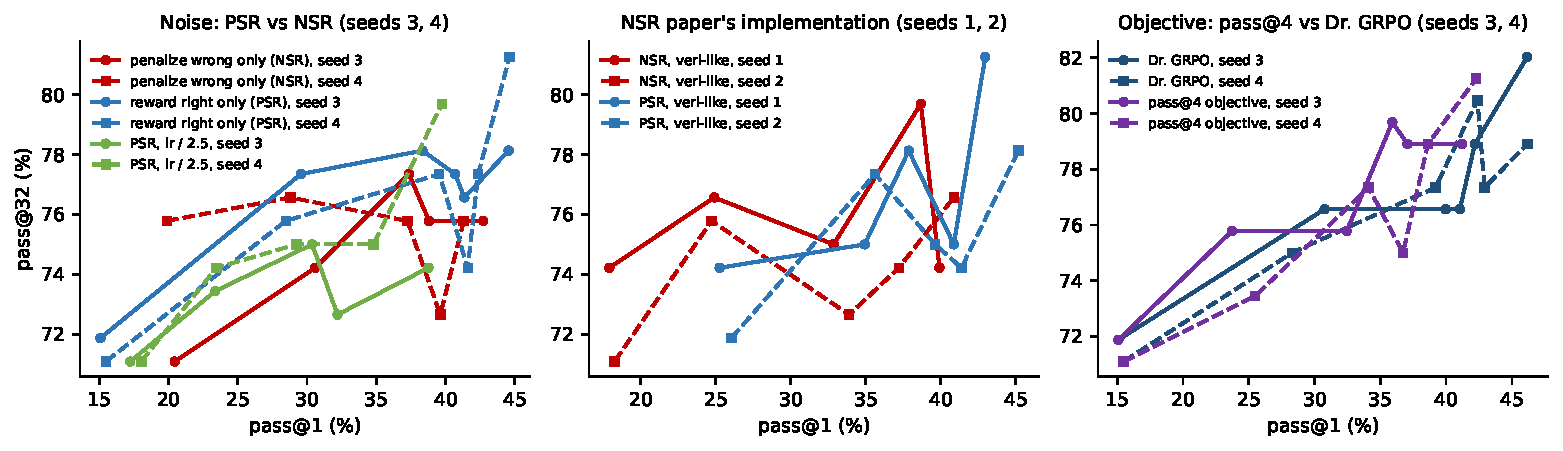
\includegraphics[width=0.9\linewidth]{frontier.pdf}\\[2pt]
\small NSR, the NSR paper's own implementation, and a pass@4 objective: all on one curve.
\end{frame}

\begin{frame}{Diagnosis 2: replicated on a second family (OLMo-2-1B)}
\centering\includegraphics[width=0.8\linewidth]{olmo_curves.pdf}\\
\small NSR vs PSR at matched accuracy: $-0.30$, 90\% $[-1.28, +0.77]$: \textbf{equivalent within $\pm2$}. NSR 19--22$\times$ noisier.
\end{frame}

\begin{frame}{Diagnosis 3: the noise is the cause}
\begin{columns}
\column{0.55\linewidth}
\includegraphics[width=\linewidth]{noise_test.pdf}
\column{0.45\linewidth}
\small
\begin{itemize}
\item Add random-sign noise of NSR's size to PSR (same mean).
\item \textbf{PSR + noise is as slow as NSR}: $\phi=-0.11$ $[-0.22,-0.05]$ (NSR $=0$, PSR $=1$).
\item NSR at 2$\times$ learning rate recovers the lag.
\item All on one curve (equivalent within $\pm2$, 3 fresh seeds).
\item Adam: noise does not shrink the steps, it misdirects them.
\end{itemize}
\end{columns}
\end{frame}

\begin{frame}{Diagnosis 4: not a temperature effect}
\begin{columns}
\column{0.45\linewidth}
\includegraphics[width=\linewidth]{temperature.pdf}
\column{0.55\linewidth}
\small
\begin{itemize}
\item On fixed text, entropy barely changes (1.081 $\to$ 1.064); on own samples it falls 3--4$\times$: RL steers into confident paths.
\item A late checkpoint at a raised temperature does \textbf{not} beat the training curve ($D=-1.42$ on 511 problems; 0.0 at the entropy-matched temperature).
\item RL is far above anything temperature does for the base model: RL adds ability.
\end{itemize}
\end{columns}
\end{frame}

\begin{frame}{What the diagnosis says a method must do}
\small
\begin{tabular}{@{}p{0.5\linewidth}p{0.44\linewidth}@{}}
\toprule
Finding & Requirement\\
\midrule
Correctness-only rules share one curve & bring information the samples lack\\
Diversity $=$ spread of success across questions & raise rarely solved questions\\
Rarely solved: groups of 8 are all wrong & supply signal there\\
No global sharpening; entropy control blocks learning & do not regulate entropy\\
Noise slows learning & keep Dr.\ GRPO as the base\\
\bottomrule
\end{tabular}
\vspace{6pt}
\begin{block}{Method: coverage-weighted success replay}
Store verified successes; each step replay 8 questions, sampled $\propto k\,p(1-p)^{k-1}=\partial\,\mathrm{pass@}k/\partial\log p$: the questions whose pass@$k$ can still rise.
\end{block}
\end{frame}

\begin{frame}{Pilot (1 seed, validation): memory is the only family that lifts}
\small\centering
\begin{tabular}{@{}lccc@{}}
\toprule
Arm & pass@1 & pass@16 & gain at matched accuracy\\
\midrule
Coverage memory $\lambda=1$ & 35.8 & 73.3 & \textcolor{good}{$+2.1$}\\
Uniform memory $\lambda=1$ & 38.6 & 72.4 & $+0.2$\\
Uniform memory $\lambda=4$ & 35.3 & 74.2 & $+3.2$ (too slow; excluded)\\
Entropy bonus & 38.9 & 72.7 & $\approx0$\\
Unlikeliness reward & 38.7 & 71.7 & $\approx-0.5$\\
Adaptive entropy & 25.5 & 65.0 & \textcolor{bad}{$-2.5$}\\
Early-token entropy floor & 12.8 & 56.1 & \textcolor{bad}{collapsed}\\
\bottomrule
\end{tabular}
\end{frame}

\begin{frame}{Main runs: interim (3 fresh seeds, 511 test problems)}
\small
\begin{itemize}
\item \textbf{Training done} (12 runs): all four arms train equally (training accuracy 60--63, greedy MATH-500 43--47).
\item \textbf{Evaluation in progress} (seed 10 so far):
\end{itemize}
\centering
\resizebox{\linewidth}{!}{\begin{tabular}{@{}lccl@{}}
\toprule
Seed 10 & pass@1 & pass@16 & vs Dr.\ GRPO (incl.\ best temperature)\\
\midrule
Dr.\ GRPO, step 50 / 100 / 150 & 37.3 / 40.6 / 44.6 & 72.4 / 71.9 / 75.2 & reference; greedy test 48.2\%\\
Coverage memory, step 50 & 36.4 & 71.8 & $-0.2$\\
Coverage memory, step 100 & 39.6 & 72.9 & $+0.3$\\
\bottomrule
\end{tabular}}
\begin{itemize}
\item Interim: \textbf{no lift yet in this seed}; the verdict needs all 3 seeds (9 points).
\end{itemize}
\end{frame}

\begin{frame}{Where we stand}
\small
\begin{tabular}{@{}lll@{}}
\toprule
Stage & Independent review (Codex) & Why\\
\midrule
Qwen only & 4/10 & claims too broad, cause not shown\\
+ noise is the cause & 5/10 & causal test passed\\
+ OLMo replication & \textbf{6/10 (weak accept)} & same curve on a second family\\
Target & 7/10 & a method that moves the curve, replicated\\
\bottomrule
\end{tabular}
\vspace{6pt}
\begin{itemize}
\item \textbf{If memory moves the curve:} OLMo replication, then the full ICML paper.
\item \textbf{If not:} a strong diagnostic paper, with an audit showing that the popular diversity fixes (NSR, entropy control, unlikeliness, pass@$k$ weights) do not move the curve, and why.
\item ICML 2027 (deadline usually late January); draft in \texttt{paper/icml/}.
\end{itemize}
\end{frame}

\end{document}
